% !TEX root = ../thesis.tex

In this thesis we consider sampling or approximating distributions that factorise in a specific way. In this chapter, we cover the Local Bouncy Particle Sampler (LBPS), a version of the BPS introduced at point \ref{point:BPS} for target distributions that factorise according to a MRF.

The aim of this short chapter is to show that the LBPS algorithm can be used on high-dimensional models such as probabilistic matrix factorisation and performances are not far those of the HMC algorithm thereby showing the potential of PDMP samplers on complex Machine Learning models. For this, we used our open-source package \texttt{PDMP.jl} coded in Julia.\footnote{\url{https://github.com/alan-turing-institute/PDMP.jl}} 

\section{Local Bouncy Particle Sampler}
In \cite{bouchard15}, the authors consider the case where the target distribution factorises as
%
\eqa{
	\pi(x)&\propto& \prod_{f\in F} \gamma_{f}(x_{f})
}
%
where $x_{f}$ is a restriction to a few elements of $x$ and $F$ is a set of \emph{factors}. In the specific case of a pairwise MRF, the factors are the edges of the graph and the restrictions are the variables corresponding to each nodes. The energy associated to $\pi$ consequently decomposes as $U\equiv \sum_{f\in F}U_{f}$.

%\subsection{Local BPS: algorithm}
For each factor, a local intensity $\lambda_{f}$ and a local bouncing operator $R_{f}$ can be defined in the same way as for the Bouncy Particle Sampler (BPS, see point \ref{point:BPS}) except that $\nabla U_{f}$ is set to have zero components for all variables not associated to the factor. We can then define a collection of intensities with
%
\eqa{
	\chi_{f}(t) &=& \lambda_{f}(x^{(i-1)}+v^{(i-1)}t,v^{(i-1)}). 
}
%
and consider the superposition principle with $\chi\equiv\sum_{f} \chi_{f}$.

Instead of modifying all velocity variables at a bounce as in the basic BPS, the method samples a factor $f$ with probability $\chi_{f}(\tau)/\chi(\tau)$ and modifies only the variables connected to the sampled factor. 
This can significantly reduce the overall computational cost associated with the algorithm and especially so when the underlying MRF has a connection structure that is not too densely connected. Indeed, when an update is triggered at a factor $f$ all factors that share a variable with $f$ are also triggered. If that corresponds to a large portion of the graph, computational gains are lost compared to simply using the full BPS. The algorithm is described in full in \citep[chapter 3.3]{bouchard15}.

%\subsection{Local BPS Algorithm}
%
%\begin{algorithm}[!h]\small
%	\caption{\label{alg:LBPS}\small \idblue{Local BPS with Priority Queue}}
%	\begin{algorithmic}[1]
%	\State initialise $(x^{(0)},v^{(0)})$, set $t_{\text{clock}}=0$
%	\State simulate a first arrival time $\tau_{\text{bounce}}^{f}\sim \text{PP}(\chi_{f}(t))$ for each factor $f$
%	\State initialise a priority queue $Q$ with the couples $\{(\tau_{f}, f)\}_{f\in F}$
%	\State initialise event lists $L_{f}$ for each factor with $(x^{(0)}_{f}, v^{(0)}_{f}, 0)$
%	\State sample $\tau_{\text{ref}}\sim\mathrm{Exp}(\lambda_{\text{ref}})$
%	\While{more events requested}
%		\State pop $(\tau_{f}, f)$ from $Q$ based on the smallest bounce time
%		\If{$\tau_{f}>\tau_{\text{ref}}$} 
%			\State $t_{\text{clock}}\leftarrow t_{\text{clock}}+\tau_{\text{ref}}$
%			\State sample a new $v\sim \mathcal N(0, \mathbb I)$
%			\State start a new queue $Q$ where the positions for each factor is extrapolated linearly until the refreshment time
%		\Else
%			\State $t_{\text{clock}}\leftarrow t_{\text{clock}}+\tau_{f}$
%			\State extrapolate $x_{f}$ linearly until $t_{\text{clock}}$
%			\State 
%		\EndIf
%	\EndWhile
%	\end{algorithmic}
%\end{algorithm}



\section{Probabilistic Matrix Factorisation}

Probabilistic Matrix Factorisation (PMF) \citep{mnih08} is a Bayesian approach to the matrix completion problem. In that problem, we consider a matrix $R$ of size $n\times p$ of ratings $r_{ij}$ corresponding to user $i$ and item $j$ (e.g.: a movie) but we only have access to a mask of $R$, a very sparse subset of the ratings which we denote $\hat R$. The aim of matrix completion methods such as PMF is to try to construct a low-rank factorisation  $R\approx U^{t}V$ based on the known entries where $U$ is of size $d\times n$ and $V$ of size $n\times p$ and $d$ is very small compared to $n$ or $p$. 

\subsection{Description of the  Model}

The model described in \citep{mnih08} assumes that each rating $r_{ij}$ is a realisation from a Normal random variable with mean $\scal{u_{i}, v_{j}}$ and standard deviation $\sigma_{r}$. 
Further, the model assumes spherical Gaussian priors on all $u_{i}$ and $v_{j}$ with standard deviation $\sigma_{u}$ and $\sigma_{v}$ respectively. Formally:
%
\begin{eqnarray}
	r_{ij} &\sim& \mathcal N(\,\cdot\, ; \scal{u_{i}, v_{j}}, \sigma_{r}), \qquad (i,j)\in\mathcal M\nn\\
	u_{i} &\sim& \mathcal N(\,\cdot\, ; 0_{d}, \sigma_{u}\mathbb I_{d}), \qquad i\in 1,\dots,n \label{eq:pmf-model}\\
	v_{j} &\sim& \mathcal N(\,\cdot\, ; 0_{d}, \sigma_{v}\mathbb I_{d}), \qquad j\in 1,\dots,p\nn
\end{eqnarray}
%
where $\mathcal M$ denotes the entries which are available, $0_{d}$ and $\mathbb I_{d}$ denote the zero vector in $\mathbb R^{d}$ and the $d\times d$ identity matrix respectively. In our experiments, we assume $\sigma_{r}, \sigma_{u}$ and $\sigma_{v}$ are fixed,\footnote{In practice, we compute sensible estimates from the data following the authors' original code available at \url{http://www.cs.toronto.edu/~rsalakhu/BPMF.html}.} more involved models exist including hyper-priors which we will not consider here since our aim is primarily to compare Local BPS and HMC on a large scale model rather than produce the best performing PMF method.\footnote{In \citep{mnih08} also suggest doing a few steps of Gibbs sampling for the hyperparameters. We do not do this in order to simplify the computations and the comparisons.}

Finally, note that the full dimensionality of the model is $n\times d + p\times d$. Below we consider an example where $d=10$, $n=6000$, $p=4000$ and $|\mathcal M|=10^{6}$ meaning that the full dimensionality of the model is $100 000$ with 1 million factors. For that kind of scale, a method such as naive Gibbs sampling (see point \ref{point:classical-sampling}) is impractical. 


\subsection{Local BPS for the PMF}

The factor graph corresponding to the matrix factorisation problem has a simple structure: each rating $r_{ij}$ for $(i,j)\in\mathcal M$ corresponds to a factor connected to the variables $u_{i}$ and $v_{j}$. This is illustrated at the figure \ref{fig:pmf-graph} below.

\begin{figure}[!h]
\center
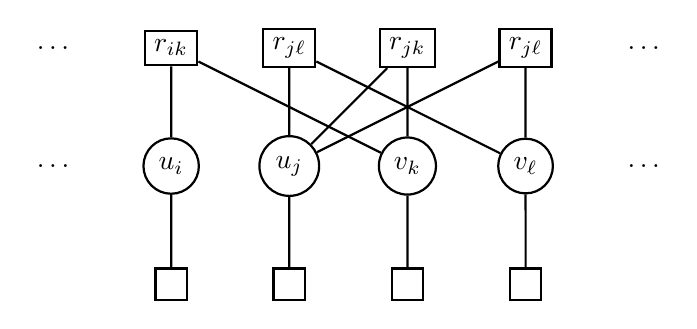
\begin{tikzpicture}[-,minimum size=.4cm,scale=.1,node distance=1.5cm, thick]
	\node[]				(A0)				{$\dots$};
	\node[rectangle,draw]	(A) [right of=A0]	{$r_{ik}$};
	\node[rectangle,draw] 	(B) [right of=A]		{$r_{j\ell}$};
	\node[rectangle,draw]	(C) [right of=B]		{$r_{jk}$};
	\node[rectangle,draw]	(E) [right of=C]		{$r_{j\ell}$};
	\node[] 				(D) [right of=E]  	{$\dots$};
	\node[circle,draw] 		(F1) [below of=A] 	{$u_{i}$};
	\node[circle,draw] 		(F2) [below of=B] 	{$u_{j}$};
	\node[circle,draw] 		(F3) [below of=C] 	{$v_{k}$};
	\node[circle,draw] 		(F4) [below of=E] 	{$v_{\ell}$};
	\node[] 				(F5) [right of=F4] 	{$\dots$};
	\node[]				(F6) [left of=F1]		{$\dots$};
	\node[rectangle,draw]	(G1)[below of=F1] 	{};
	\node[rectangle,draw]	(G2)[below of=F2] 	{};
	\node[rectangle,draw]	(G3)[below of=F3] 	{};
	\node[rectangle,draw]	(G4)[below of=F4] 	{};
	\path 
	(A) edge	(F1)
	(A) edge	(F3)
	(B) edge	(F2)
	(B) edge 	(F4)
	(C) edge 	(F2)
	(C) edge 	(F3)
	(E) edge 	(F2)
	(E) edge	(F4)
	(G1) edge (F1)
	(G2) edge (F2)
	(G3) edge (F3)
	(G4) edge (F4)
	;
\end{tikzpicture}
\caption{\label{fig:pmf-graph} Illustration of the factor-graph corresponding to the matrix completion problem. Each observed rating corresponds to a factor connected to a corresponding $u$-node and $v$-node themselves corresponding to $d$-dimensional variables. Each node also has its own factor corresponding to a spherical Gaussian prior (empty squares).}
\end{figure} 

% Note that while every rating factor has degree 2 in the graph whereas it can vary for each variable nodes.  

The energy associated with one of the rating factor is also easily obtained by taking the negative log-likelihood associated to $r_{ij}$ (see \eqref{eq:pmf-model}), we denote it $\mathcal E_{ij}$ with
%
\eqa{
	\mathcal E_{ij}(u_{i}, v_{j}) &:=& 0.5\sigma_{r}^{-2}(r_{ij}-\scal{u_{i}, v_{j}})^{2}.
}
%
Correspondingly, the prior-factors are associated with $\mathcal E^{u}_{i}(u_{i}):=0.5\sigma_{u}^{-2}\|u_{i}\|_{2}^{2}$ and $\mathcal E^{v}_{j}(v_{j}):=0.5\sigma_{v}^{-2}\|v_{j}\|_{2}^{2}$. The Inhomogeneous Poisson Processes (IPP) associated with Gaussians can easily be sampled from using the inversion method. 
The IPP associated with the rating factors can also be easily sampled from using the inversion method which we show below.

\subsubsection{Sampling the IPP associated with a rating factor}

To simplify notations, we consider a single rating $r$ associated with two $d$-dimensional vectors $u$ and $v$. We introduce the notation $x:=(u; v)$ and write $x_{u}=u$ and $x_{v}=v$. We also write $e(x):=(\scal{x_{u},x_{v}}-r)$. With these notations, we can write the energy as $\mathcal E(x) = 0.5\sigma_{r}^{-2}e^{2}(x)$. 
As for the BPS, the intensity associated with this factor is $\chi(t) = \scal{\nabla \mathcal E(x+tw), w}^{+}$ where $w$ is a velocity-vector of the same dimension as $x$. The gradient with respect to the $u$ and $v$ component can be written as
\eqa{
	\syst{\nabla_{x_{u}} \mathcal E(x) &=& \gamma(x)x_{v}\\
		\nabla_{x_{v}} \mathcal E(x) &=& \gamma(x)x_{u}}
}
where $\gamma(x):=\sigma_{r}^{-2}e(x)$. It is straightforward to show that the inner product \\$\scal{\nabla\mathcal E(x+tw), w}$ is a third-order polynomial in $t$ with
\eqa{
	\scal{\nabla\mathcal E(x+tw), w} &=& \gamma(x+tw)\pac{\scal{x_{u},w_{v}} + \scal{x_{v}, w_{u}} + 2t\scal{w_{u}, w_{v}}} \label{ipp-3dorder}
}
The intensity $\chi(t)$ of the IPP is therefore given by the positive part of this third-order polynomial. The factor of $t^{3}$ in \eqref{ipp-3dorder} is positive which is already indicative of the shape of the polynomial but the roots of the polynomial need to be studied in order to fully characterise it. It is easy to obtain the root corresponding to the left-parenthesis in \eqref{ipp-3dorder} which we denote $t_{0}$ with $t_{0}=-d(x,w)/2s(w)$ where $d(x,w):=(\scal{x_{u}, w_{v}}+\scal{x_{v},w_{u}})$ and $s(w):=\scal{w_{u},w_{v}}$. The other two roots are obtained by setting $\gamma(x+tw)$ or equivalently $e(x+tw)$ to zero. All the roots of \eqref{ipp-3dorder} are therefore given by:
\eqa{
	\syst{	t_{0} &=& -d(x,w)/2s(w)\\
			t_{-,+} &=& t_{0} \pm \sqrt{t_{0}^{2}+e(x)/s(w)}	}.
}

Using the inversion method, sampling from the IPP can be done in two steps: generate a $\lambda\sim\mathrm{Exp}(1)$ and then find $t(\lambda)$ such that
\eqa{
	\lambda \spe \Xi(t(\lambda)) &=& \int_{0}^{t(\lambda)} \chi(s)\ds.
}
Since $\chi(t)$ is the positive part of a third-order polynomial, the integral can be computed exactly and the inversion to obtain $t(\lambda)$ amounts to finding a root of a fourth-order polynomial which can be done efficiently using a numerical solver. 

%\mathcal{}


\subsection{Other algorithms considered}

\subsubsection{Singular Value Decomposition}

As a baseline, we consider the Singular Value Decomposition (SVD) algorithm. Indeed, Eckart and Young's theorem shows that for a matrix $M$, the truncated SVD is the best low-rank approximation in the sense of the Frobenius norm. In the matrix completion case, no guarantees are offered by the SVD since we only have access to a sparse mask of the real matrix \citep{srebro04}. Let $R$ denote the true matrix we are trying to reconstruct and $\hat R$ the sparse matrix containing only the observed ratings (centred). The SVD decomposition of $\hat R$ gives $\hat R = U\Sigma V^{t}$ where $U$ is an orthonormal matrix of size $n\times p$, $\Sigma$ is a diagonal matrix of size $p\times p$ and $V$ is an orthogonal matrix of size $p\times p$. Truncating $\Sigma$ to its first $d\ll p$ components leads to a rank-$d$ approximation $\tilde R$ to $\hat R$. 
Letting $U_{\text{SVD}}:=\Sigma^{1/2}U^{t}$ and $V_{\text{SVD}}:=\Sigma^{1/2}V^{t}$ we have a first baseline factorisation $\tilde R=U_{\text{SVD}}^{t}V_{\text{SVD}}\approx R$.

Note that the problem of computing a truncated SVD decomposition of a large sparse system is a well known problem in numerical linear algebra and very efficient methods exist \citep{sorensen96}.\footnote{In the experiments, we use the \texttt{svds} function from Julia 0.6 uses the implicitly restarted Lanczos iterations.}

\subsubsection{Hamiltonian Monte Carlo}

The negative log posterior in $U$ and $V$ of the model can be directly obtained:
\eqa{
	-2\log p (U, V | \hat R) &=& \sigma_{r}^{-2}\sum_{(i,j)\in\mathcal M} (r_{ij}-\scal{u_{i},v_{j}})^{2} +\sigma_{u}^{-2}\|U\|_{2}^{2} + \sigma_{v}^{-2}\|V\|_{2}^{2}.\nn
}
Therefore, the gradient in $u_{i}$ and $v_{j}$ can easily be computed in closed form and it is straightforward to apply HMC on this model (cf.\ algorithm \ref{alg:hmc-alg}). The main hurdle is that each gradient evaluation requires a full pass over all observed ratings. 

\subsection{Experiments}

In our experiments, we consider the MovieLens 1M dataset.\footnote{\url{https://grouplens.org/datasets/movielens/}} corresponding to 1 million ratings of 4000 movies by 6000 users. We take a random subset of 80\% of the ratings as training set using the remaining 20\% as test set.


\section{Discussion}










